\documentclass{article}
\usepackage{tikz}
\usetikzlibrary{arrows.meta}

\begin{document}

\begin{figure}[h]
    \centering
    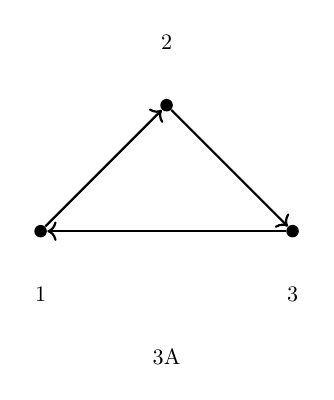
\begin{tikzpicture}[scale=0.8, every node/.style={scale=0.8}]
        % Node definitions
        \node (1) at (0, 0) [circle, fill, inner sep=2pt] {};
        \node (2) at (2, 2) [circle, fill, inner sep=2pt] {};
        \node (3) at (4, 0) [circle, fill, inner sep=2pt] {};
        
        % Edges
        \draw[->, thick] (1) -- (2);
        \draw[->, thick] (2) -- (3);
        \draw[->, thick] (3) -- (1);
        
        \node at (0,-1) {1};
        \node at (2, 3) {2};
        \node at (4,-1) {3};
        
        \node at (2,-2) {3A};
    \end{tikzpicture}
    
    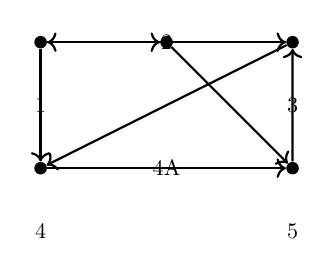
\begin{tikzpicture}[scale=0.8, every node/.style={scale=0.8}]
        % Node definitions
        \node (1) at (0, 0) [circle, fill, inner sep=2pt] {};
        \node (2) at (2, 0) [circle, fill, inner sep=2pt] {};
        \node (3) at (4, 0) [circle, fill, inner sep=2pt] {};
        \node (4) at (0, -2) [circle, fill, inner sep=2pt] {};
        \node (5) at (4, -2) [circle, fill, inner sep=2pt] {};
        
        % Edges
        \draw[->, thick] (1) -- (2);
        \draw[->, thick] (2) -- (3);
        \draw[->, thick] (3) -- (1);
        \draw[->, thick] (1) -- (4);
        \draw[->, thick] (2) -- (5);
        \draw[->, thick] (3) -- (4);
        \draw[->, thick] (4) -- (5);
        \draw[->, thick] (5) -- (3);
        
        \node at (0,-1) {1};
        \node at (2, 0) {2};
        \node at (4,-1) {3};
        \node at (0,-3) {4};
        \node at (4,-3) {5};
        
        \node at (2,-2) {4A};
    \end{tikzpicture}
    
    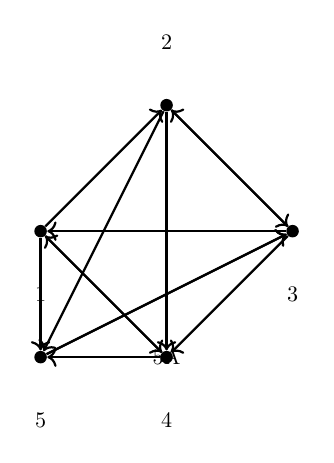
\begin{tikzpicture}[scale=0.8, every node/.style={scale=0.8}]
        % Node definitions
        \node (1) at (0, 0) [circle, fill, inner sep=2pt] {};
        \node (2) at (2, 2) [circle, fill, inner sep=2pt] {};
        \node (3) at (4, 0) [circle, fill, inner sep=2pt] {};
        \node (4) at (2, -2) [circle, fill, inner sep=2pt] {};
        \node (5) at (0, -2) [circle, fill, inner sep=2pt] {};
        
        % Edges
        \draw[->, thick] (1) -- (2);
        \draw[->, thick] (2) -- (3);
        \draw[->, thick] (3) -- (1);
        \draw[->, thick] (1) -- (4);
        \draw[->, thick] (2) -- (5);
        \draw[->, thick] (3) -- (4);
        \draw[->, thick] (4) -- (5);
        \draw[->, thick] (5) -- (3);
        \draw[->, thick] (1) -- (5);
        \draw[->, thick] (2) -- (4);
        \draw[->, thick] (3) -- (2);
        \draw[->, thick] (4) -- (1);
        \draw[->, thick] (5) -- (3);
        
        \node at (0,-1) {1};
        \node at (2, 3) {2};
        \node at (4,-1) {3};
        \node at (2,-3) {4};
        \node at (0,-3) {5};
        
        \node at (2,-2) {5A};
    \end{tikzpicture}
    
    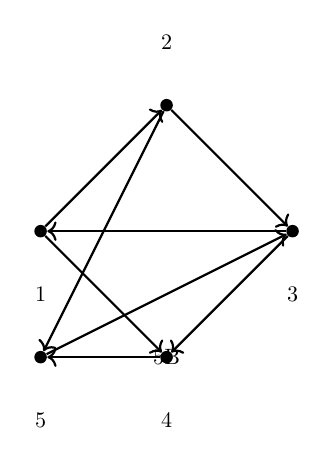
\begin{tikzpicture}[scale=0.8, every node/.style={scale=0.8}]
        % Node definitions
        \node (1) at (0, 0) [circle, fill, inner sep=2pt] {};
        \node (2) at (2, 2) [circle, fill, inner sep=2pt] {};
        \node (3) at (4, 0) [circle, fill, inner sep=2pt] {};
        \node (4) at (2, -2) [circle, fill, inner sep=2pt] {};
        \node (5) at (0, -2) [circle, fill, inner sep=2pt] {};
        
        % Edges
        \draw[->, thick] (1) -- (2);
        \draw[->, thick] (2) -- (3);
        \draw[->, thick] (3) -- (1);
        \draw[->, thick] (1) -- (4);
        \draw[->, thick] (2) -- (5);
        \draw[->, thick] (3) -- (4);
        \draw[->, thick] (4) -- (5);
        \draw[->, thick] (5) -- (3);
        
        \node at (0,-1) {1};
        \node at (2, 3) {2};
        \node at (4,-1) {3};
        \node at (2,-3) {4};
        \node at (0,-3) {5};
        
        \node at (2,-2) {5B};
    \end{tikzpicture}
    
    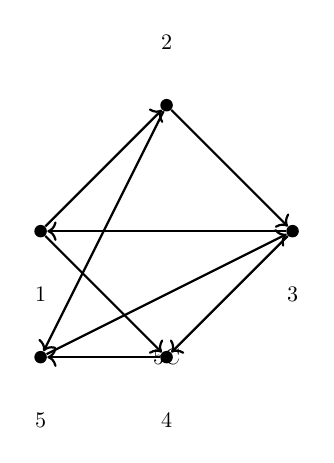
\begin{tikzpicture}[scale=0.8, every node/.style={scale=0.8}]
        % Node definitions
        \node (1) at (0, 0) [circle, fill, inner sep=2pt] {};
        \node (2) at (2, 2) [circle, fill, inner sep=2pt] {};
        \node (3) at (4, 0) [circle, fill, inner sep=2pt] {};
        \node (4) at (2, -2) [circle, fill, inner sep=2pt] {};
        \node (5) at (0, -2) [circle, fill, inner sep=2pt] {};
        
        % Edges
        \draw[->, thick] (1) -- (2);
        \draw[->, thick] (2) -- (3);
        \draw[->, thick] (3) -- (1);
        \draw[->, thick] (1) -- (4);
        \draw[->, thick] (2) -- (5);
        \draw[->, thick] (3) -- (4);
        \draw[->, thick] (4) -- (5);
        \draw[->, thick] (5) -- (3);
        
        \node at (0,-1) {1};
        \node at (2, 3) {2};
        \node at (4,-1) {3};
        \node at (2,-3) {4};
        \node at (0,-3) {5};
        
        \node at (2,-2) {5C};
    \end{tikzpicture}
    
    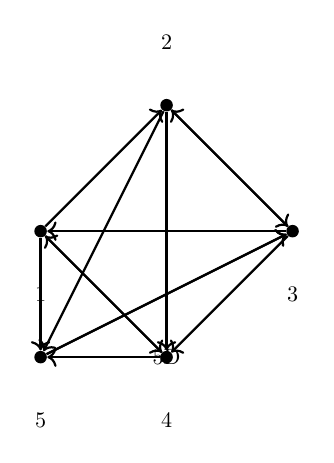
\begin{tikzpicture}[scale=0.8, every node/.style={scale=0.8}]
        % Node definitions
        \node (1) at (0, 0) [circle, fill, inner sep=2pt] {};
        \node (2) at (2, 2) [circle, fill, inner sep=2pt] {};
        \node (3) at (4, 0) [circle, fill, inner sep=2pt] {};
        \node (4) at (2, -2) [circle, fill, inner sep=2pt] {};
        \node (5) at (0, -2) [circle, fill, inner sep=2pt] {};
        
        % Edges
        \draw[->, thick] (1) -- (2);
        \draw[->, thick] (2) -- (3);
        \draw[->, thick] (3) -- (1);
        \draw[->, thick] (1) -- (4);
        \draw[->, thick] (2) -- (5);
        \draw[->, thick] (3) -- (4);
        \draw[->, thick] (4) -- (5);
        \draw[->, thick] (5) -- (3);
        \draw[->, thick] (1) -- (5);
        \draw[->, thick] (2) -- (4);
        \draw[->, thick] (3) -- (2);
        \draw[->, thick] (4) -- (1);
        \draw[->, thick] (5) -- (3);
        
        \node at (0,-1) {1};
        \node at (2, 3) {2};
        \node at (4,-1) {3};
        \node at (2,-3) {4};
        \node at (0,-3) {5};
        
        \node at (2,-2) {5D};
    \end{tikzpicture}
    
    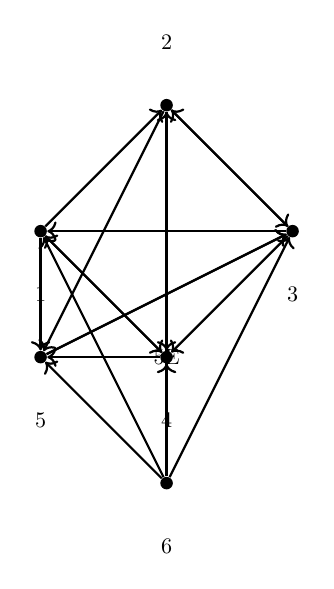
\begin{tikzpicture}[scale=0.8, every node/.style={scale=0.8}]
        % Node definitions
        \node (1) at (0, 0) [circle, fill, inner sep=2pt] {};
        \node (2) at (2, 2) [circle, fill, inner sep=2pt] {};
        \node (3) at (4, 0) [circle, fill, inner sep=2pt] {};
        \node (4) at (2, -2) [circle, fill, inner sep=2pt] {};
        \node (5) at (0, -2) [circle, fill, inner sep=2pt] {};
        \node (6) at (2, -4) [circle, fill, inner sep=2pt] {};
        
        % Edges
        \draw[->, thick] (1) -- (2);
        \draw[->, thick] (2) -- (3);
        \draw[->, thick] (3) -- (1);
        \draw[->, thick] (1) -- (4);
        \draw[->, thick] (2) -- (5);
        \draw[->, thick] (3) -- (4);
        \draw[->, thick] (4) -- (5);
        \draw[->, thick] (5) -- (3);
        \draw[->, thick] (1) -- (5);
        \draw[->, thick] (2) -- (4);
        \draw[->, thick] (3) -- (2);
        \draw[->, thick] (4) -- (1);
        \draw[->, thick] (5) -- (3);
        \draw[->, thick] (6) -- (1);
        \draw[->, thick] (6) -- (2);
        \draw[->, thick] (6) -- (3);
        \draw[->, thick] (6) -- (4);
        \draw[->, thick] (6) -- (5);
        
        \node at (0,-1) {1};
        \node at (2, 3) {2};
        \node at (4,-1) {3};
        \node at (2,-3) {4};
        \node at (0,-3) {5};
        \node at (2,-5) {6};
        
        \node at (2,-2) {5E};
    \end{tikzpicture}
    
    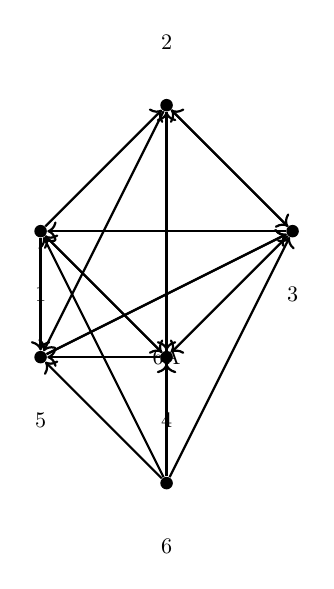
\begin{tikzpicture}[scale=0.8, every node/.style={scale=0.8}]
        % Node definitions
        \node (1) at (0, 0) [circle, fill, inner sep=2pt] {};
        \node (2) at (2, 2) [circle, fill, inner sep=2pt] {};
        \node (3) at (4, 0) [circle, fill, inner sep=2pt] {};
        \node (4) at (2, -2) [circle, fill, inner sep=2pt] {};
        \node (5) at (0, -2) [circle, fill, inner sep=2pt] {};
        \node (6) at (2, -4) [circle, fill, inner sep=2pt] {};
        
        % Edges
        \draw[->, thick] (1) -- (2);
        \draw[->, thick] (2) -- (3);
        \draw[->, thick] (3) -- (1);
        \draw[->, thick] (1) -- (4);
        \draw[->, thick] (2) -- (5);
        \draw[->, thick] (3) -- (4);
        \draw[->, thick] (4) -- (5);
        \draw[->, thick] (5) -- (3);
        \draw[->, thick] (1) -- (5);
        \draw[->, thick] (2) -- (4);
        \draw[->, thick] (3) -- (2);
        \draw[->, thick] (4) -- (1);
        \draw[->, thick] (5) -- (3);
        \draw[->, thick] (6) -- (1);
        \draw[->, thick] (6) -- (2);
        \draw[->, thick] (6) -- (3);
        \draw[->, thick] (6) -- (4);
        \draw[->, thick] (6) -- (5);
        
        \node at (0,-1) {1};
        \node at (2, 3) {2};
        \node at (4,-1) {3};
        \node at (2,-3) {4};
        \node at (0,-3) {5};
        \node at (2,-5) {6};
        
        \node at (2,-2) {6A};
    \end{tikzpicture}
    
    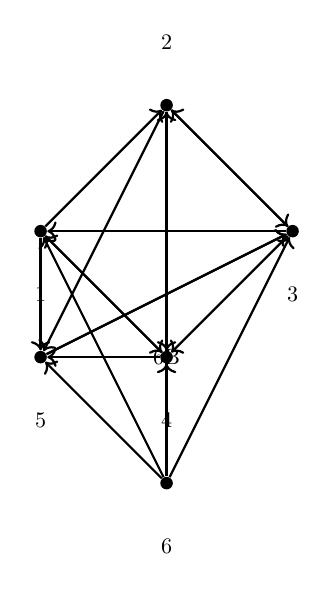
\begin{tikzpicture}[scale=0.8, every node/.style={scale=0.8}]
        % Node definitions
        \node (1) at (0, 0) [circle, fill, inner sep=2pt] {};
        \node (2) at (2, 2) [circle, fill, inner sep=2pt] {};
        \node (3) at (4, 0) [circle, fill, inner sep=2pt] {};
        \node (4) at (2, -2) [circle, fill, inner sep=2pt] {};
        \node (5) at (0, -2) [circle, fill, inner sep=2pt] {};
        \node (6) at (2, -4) [circle, fill, inner sep=2pt] {};
        
        % Edges
        \draw[->, thick] (1) -- (2);
        \draw[->, thick] (2) -- (3);
        \draw[->, thick] (3) -- (1);
        \draw[->, thick] (1) -- (4);
        \draw[->, thick] (2) -- (5);
        \draw[->, thick] (3) -- (4);
        \draw[->, thick] (4) -- (5);
        \draw[->, thick] (5) -- (3);
        \draw[->, thick] (1) -- (5);
        \draw[->, thick] (2) -- (4);
        \draw[->, thick] (3) -- (2);
        \draw[->, thick] (4) -- (1);
        \draw[->, thick] (5) -- (3);
        \draw[->, thick] (6) -- (1);
        \draw[->, thick] (6) -- (2);
        \draw[->, thick] (6) -- (3);
        \draw[->, thick] (6) -- (4);
        \draw[->, thick] (6) -- (5);
        
        \node at (0,-1) {1};
        \node at (2, 3) {2};
        \node at (4,-1) {3};
        \node at (2,-3) {4};
        \node at (0,-3) {5};
        \node at (2,-5) {6};
        
        \node at (2,-2) {6B};
    \end{tikzpicture}
    \caption{Sample Graphs}
\end{figure}

\end{document}